% FILE:    thesis_main.tex 
% AUTHOR:  Symon Stowe 
% DATE:    2020-01-06
%--------------------------------------------------------
% !TEX program = lualatex
% !BIB program = biber

% Define style of document
%\documentclass[12pt,twoside]{report}
\documentclass[12pt]{report}
\usepackage{amsmath} 

% BIBER
\usepackage{csquotes}
\usepackage[american]{babel}
\usepackage[
backend=biber,
style=apa,
giveninits=true,
doi=false,
isbn=false,
url=false,
citestyle=authoryear,
maxbibnames=19,
apamaxprtauth=99,
maxcitenames=2,
uniquename=false,
uniquelist=false
]{biblatex}

\DeclareLanguageMapping{american}{american-apa}

\renewbibmacro*{name:andothers}{% Based on name:andothers from biblatex.def
  \ifboolexpr{
    test {\ifnumequal{\value{listcount}}{\value{liststop}}}
    and
    test \ifmorenames
  }
    {\ifnumgreater{\value{liststop}}{1}
       {\finalandcomma}
       {}%
     \andothersdelim\bibstring[\emph]{andothers}}
    {}}
\addbibresource{chapter_2/refs.bib}
\newcommand{\citeauthorandyear}[2][]{
   \citeauthor{#2} (\citeyear[#1]{#2})}
\renewcommand*{\nameyeardelim}{\addcomma\space} % Remove this line if you don't want the comma in citations

% Shortcuts for the perfusion paper
\newcommand{\PVi}{{\rm P_{Vf}}}
\newcommand{\PAa}{{\rm P_{At}}}
\newcommand{\PAi}{{\rm P_{Af}}}
\newcommand{\PVa}{{\rm P_{Vt}}}
\newcommand{\PBi}{{\rm P_{B}}}
\newcommand{\yB}{\mathbf{y}}
\newcommand{\vB}{\mathbf{v}}
\newcommand{\uB}{\mathbf{u}}
\newcommand{\xB}{\mathbf{x}}
\newcommand{\xH}{\hat{\mathbf{x}}}
\newcommand{\nB}{\mathbf{n}}
\newcommand{\CB}{\mathbf{C}}
\newcommand{\FB}{\mathbf{F}}
\newcommand{\JB}{\mathbf{J}}
\newcommand{\DB}{\mathbf{D}}
\newcommand{\EX}{\mathrm{E}}
\newcommand{\IB}{\mathbf{I}}
\newcommand{\LB}{\mathbf{L}}
\newcommand{\MB}{\mathbf{M}}
\newcommand{\RB}{\mathbf{R}}
\newcommand{\qB}{\mathbf{q}}
\newcommand{\QB}{\mathbf{Q}}
\newcommand{\VB}{\mathbf{V}}
\newcommand{\WB}{\mathbf{W}}
\newcommand{\sG}{\boldsymbol{\sigma}}
\newcommand{\gG}{\boldsymbol{\gamma}}
\newcommand{\GG}{\boldsymbol{\Gamma}}
\newcommand{\SG}{\boldsymbol{\Sigma}}
\newcommand{\LG}{\boldsymbol{\Lambda}}

\usepackage{fancyref}    

% Define margins of document
\sloppy
\usepackage{geometry}
\geometry{verbose,letterpaper} %,tmargin=20mm,bmargin=20mm,lmargin=20mm,rmargin=20mm}
% TODO how to we make the margins alternate like they should be in a book?
% TODO different print vs online versions with different margins?

% Set overall spacing
\usepackage{setspace}
\doublespacing
%\onehalfspacing   

% Shrink list spacing
% shrink the list environments
\usepackage{enumitem}
\setlist{noitemsep}
\setlist{nolistsep}

% Blank pages
\usepackage{afterpage}

\newcommand\blankpage{%
    \null
    \thispagestyle{empty}%
    %\addtocounter{page}{-1}%
    \newpage}

%List of abbreviations
\usepackage[acronym,nomain,nonumberlist]{glossaries}

\newacronym{eit}{EIT}{electrical impedance tomography}
\newacronym{mse}{MSE}{mean squared error}
\newacronym{fwhm}{FWHM}{full width half max}
\newacronym{sv}{SV}{stroke volume}
\newacronym{lv}{LV}{left ventricular}
\newacronym{svv}{SVV}{stroke volume variation}
\newacronym{co}{CO}{cardiac output}
\newacronym{fem}{FEM}{finite element model}
\newacronym{ct}{CT}{computed tomography}
\newacronym{mri}{MRI}{magnetic resonance imaging}
\newacronym{ards}{ARDS}{acute respiratory distress syndrome}
\newacronym{pet}{PET}{positron emission tomography}
\newacronym{spect}{SPECT}{single photon emission computed tomography}
\makeglossaries

% Include packages for manipulating figures/tables
\usepackage{epsfig} 

% Different font size in captions
\usepackage{/Users/symonstowe/thesis/proposal/tex/ccaption}
\captionnamefont{\bf \footnotesize}
\captiontitlefont{\footnotesize}
\captionwidth{130mm}
\changecaptionwidth

% Define page numbering scheme
\pagenumbering{roman}

% Make the table of contents clickable
\usepackage{hyperref}

% For the papers in appendix
\usepackage{pdfpages}

% Start of document
\begin{document}

% Define aliases
\newcommand{\pbox}{\parbox}

% Figures and Tables
\newtheorem{fig}{Figure}
\newtheorem{tab}{Table}

% Counter commands
\setcounter{page}{1}
\setcounter{chapter}{0}
\setcounter{secnumdepth}{4}
\setcounter{tocdepth}{3}

% BODY OF TEXT 
% Include the following files in main document
\normalsize

% START OF THESIS
% TITLE PAGE
% FILE:    title.tex
% AUTHOR:  Symon Stowe 
% DATE:    2020-01-06
%--------------------------------------------------------

% Suppress page number 
\thispagestyle{empty}
\begin{center}

%\vspace{-5mm}
\LARGE

\textbf{Electrical Impedance Tomography for Perfusion Imaging and Monitoring}

\vspace{6mm}
\large
by 

\vspace{-2mm}
\LARGE
Symon Stowe

\vspace{15mm}
\large
A thesis submitted in partial fulfillment of 
the requirements for the degree of

\vspace{12mm}
\large
Ph.D.\\

in \\

\vspace{1mm}
Biomedical Engineering\\

\vspace{12mm}
\large
Carleton University \\
Ottawa, Ontario\\

\vspace{12mm}
\large
\copyright~2021 \\
Symon Stowe
\end{center}

\afterpage{\blankpage}
\phantomsection
% DEDICATION
% Suppress page number
\thispagestyle{empty}

\mbox{  }
\begin{flushright}

\vspace{6cm}
\large

\textit{To ...}
\end{flushright}

\afterpage{\blankpage}

% LIST OF ABBREVIATIONS and SYMBOLS
%\addcontentsline{toc}{chapter}{List of Abbreviations}
%% FILE:    abbrev_body.tex
% AUTHOR:  Camille Gomez-Laberge 
% DATE:    12.04.2006
%
% (C) 2006, Camille Gomez-Laberge
% $Id: abbrev_body.tex 1302 2007-07-19 14:08:08Z cgomez $
%--------------------------------------------------------

\markboth{List of Abbreviations}
         {List of Abbreviations}

\subsection*{List of Abbreviations}

% BEGIN TABLE X.X
% SUBJECT: TABLE
\begin{table}[!h]
\vspace{5mm}
{\centering
\small
\begin{tabular}[t]{|c|c|}
\hline
\pbox[t]{30mm}{\centering \textbf{Abbreviation}} &
\pbox[t]{110mm}{\centering \textbf{Details}} \\
\hline

\pbox[t]{30mm}{\raggedright ASCII}&
\pbox[t]{110mm}{\raggedright American Standard Code for Information Interchange}\\

\pbox[t]{30mm}{\raggedright BLAST}&
\pbox[t]{110mm}{\raggedright Basic Local Alignment Search Tool}\\

\pbox[t]{30mm}{\raggedright BLOSUM}&
\pbox[t]{110mm}{\raggedright Blocks Substitution Matrices}\\

\pbox[t]{30mm}{\raggedright CASP}&
\pbox[t]{110mm}{\raggedright Critical Assessment of Methods of Protein Structure Prediction}\\

\pbox[t]{30mm}{\raggedright CATH}&
\pbox[t]{110mm}{\raggedright Class, Architecture, Topology, Homologous Superfamily}\\

\pbox[t]{30mm}{\raggedright CATH-PFDB}&
\pbox[t]{110mm}{\raggedright CATH Protein Family Database}\\

\pbox[t]{30mm}{\raggedright COG}&
\pbox[t]{110mm}{\raggedright Clusters of Orthologous Groups}\\

\pbox[t]{30mm}{\raggedright CORA}&
\pbox[t]{110mm}{\raggedright Conserved Residue Attributes}\\

\pbox[t]{30mm}{\raggedright DDBJ}&
\pbox[t]{110mm}{\raggedright DNA Databank of Japan}\\

\pbox[t]{30mm}{\raggedright DHDPS}&
\pbox[t]{110mm}{\raggedright Dihydropicolinate Synthetase}\\

\pbox[t]{30mm}{\raggedright DHS}&
\pbox[t]{110mm}{\raggedright Dictionary of Homologous Superfamilies}\\

\pbox[t]{30mm}{\raggedright DIVCLUS}&
\pbox[t]{110mm}{\raggedright Divide and Cluster}\\

\pbox[t]{30mm}{\raggedright DNA}&
\pbox[t]{110mm}{\raggedright Deoxyribonucleic Acid}\\

\pbox[t]{30mm}{\raggedright DSSP}&
\pbox[t]{110mm}{\raggedright Dictionary of Protein Secondary Structures}\\

\pbox[t]{30mm}{\raggedright EBI}&
\pbox[t]{110mm}{\raggedright European Bioinformatics Institute}\\

\pbox[t]{30mm}{\raggedright EC}&
\pbox[t]{110mm}{\raggedright Enzyme Commission}\\

\pbox[t]{30mm}{\raggedright EMBL}&
\pbox[t]{110mm}{\raggedright European Molecular Biology Laboratory}\\

\pbox[t]{30mm}{\raggedright EPQ}&
\pbox[t]{110mm}{\raggedright Error Per Query}\\

\pbox[t]{30mm}{\raggedright EVD}&
\pbox[t]{110mm}{\raggedright Extreme Value Distribution}\\

\pbox[t]{30mm}{\raggedright ExPASy}&
\pbox[t]{110mm}{\raggedright Expert Protein Analysis System}\\

\pbox[t]{30mm}{\raggedright FAD}&
\pbox[t]{110mm}{\raggedright Flavin Adenine Nucleotide}\\

\pbox[t]{30mm}{\raggedright FFF}&
\pbox[t]{110mm}{\raggedright Fuzzy Functional Forms}\\

\pbox[t]{30mm}{\raggedright FOD}&
\pbox[t]{110mm}{\raggedright Frequently Occurring Domain}\\

\pbox[t]{30mm}{\raggedright FORREST}&
\pbox[t]{110mm}{\raggedright Fold Recognition from Secondary Structures}\\

\pbox[t][9mm]{30mm}{\raggedright FSSP}&
\pbox[t]{110mm}{\raggedright Fold classification based on Structure-Structure alignment of Proteins}\\

\pbox[t]{30mm}{\raggedright HMM}&
\pbox[t]{110mm}{\raggedright Hidden Markov Models}\\

%\pbox[t]{30mm}{\raggedright HOMSTRAD}&
%\pbox[t]{110mm}{\raggedright Homologous Structure Alignment Database}\\

\pbox[t]{30mm}{\raggedright HSP}&
\pbox[t]{110mm}{\raggedright High Scoring Segment Pairs}\\

\pbox[t]{30mm}{\raggedright HSSP}&
\pbox[t]{110mm}{\raggedright Homology derived Secondary Structure of Proteins}\\

\pbox[t]{30mm}{\raggedright HTML}&
\pbox[t]{110mm}{\raggedright Hypertext Markup Language}\\

\pbox[t]{30mm}{\raggedright IMPALA}&
\pbox[t]{110mm}{\raggedright Integrating Matrix Profiles And Local Alignments}\\

\pbox[t]{30mm}{\raggedright ISL}&
\pbox[t]{110mm}{\raggedright Intermediate Sequence Library}\\

\pbox[t]{30mm}{\raggedright ISS}&
\pbox[t]{110mm}{\raggedright Intermediate Sequence Search}\\

\pbox[t]{30mm}{\raggedright JIPID}&
\pbox[t]{110mm}{\raggedright Protein Information Database of Japan}\\

\pbox[t]{30mm}{\raggedright LCS}&
\pbox[t]{110mm}{\raggedright Longest Continuous Segment}\\

\pbox[t]{30mm}{\raggedright MDM}&
\pbox[t]{110mm}{\raggedright Mutation Data Matrix}\\

\pbox[t]{30mm}{\raggedright MIPS}&
\pbox[t]{110mm}{\raggedright Martinsried Institute for Protein Sequences}\\

\pbox[t]{30mm}{\raggedright MISS}&
\pbox[t]{110mm}{\raggedright Multiple Intermediate Sequence Search}\\

\pbox[t]{30mm}{\raggedright MMDB}&
\pbox[t]{110mm}{\raggedright Molecular Modelling Database}\\

\hline
\end{tabular}
\par}
\centering
\end{table}
\vspace{5mm}
% END TABLE X.X

% BEGIN TABLE X.X
% SUBJECT: TABLE
\begin{table}[!h]
\vspace{5mm}
{\centering
\small
\begin{tabular}[t]{|c|c|}
\hline
\pbox[t]{30mm}{\centering \textbf{Abbreviation}} &
\pbox[t]{110mm}{\centering \textbf{Details}} \\
\hline

\pbox[t]{30mm}{\raggedright NAD}&
\pbox[t]{110mm}{\raggedright Nicotinamide Adenine Dinucleotide}\\

\pbox[t][9mm]{30mm}{\raggedright NC-IUBMB}&
\pbox[t]{110mm}{\raggedright Nomenclature Committee of the International Union of Biochemistry and Molecular Biology}\\

\pbox[t]{30mm}{\raggedright NCBI}&
\pbox[t]{110mm}{\raggedright National Center for Biotechnology Information}\\

\pbox[t]{30mm}{\raggedright NMR}&
\pbox[t]{110mm}{\raggedright Nuclear Magnetic Resonance}\\

\pbox[t]{30mm}{\raggedright NRDB}&
\pbox[t]{110mm}{\raggedright Non-redundant Database}\\

\pbox[t]{30mm}{\raggedright ORF}&
\pbox[t]{110mm}{\raggedright Open Reading Frame}\\

\pbox[t]{30mm}{\raggedright PAM}&
\pbox[t]{110mm}{\raggedright Point Accepted Mutation}\\

\pbox[t]{30mm}{\raggedright PCA}&
\pbox[t]{110mm}{\raggedright Principal Component Analysis}\\

\pbox[t]{30mm}{\raggedright PCR}&
\pbox[t]{110mm}{\raggedright Polymerase Chain Reaction}\\

\pbox[t]{30mm}{\raggedright PDB}&
\pbox[t]{110mm}{\raggedright Protein Data Bank}\\

\pbox[t]{30mm}{\raggedright PEDANT}&
\pbox[t]{110mm}{\raggedright Protein Extraction, Description and Analysis Tool}\\

\pbox[t]{30mm}{\raggedright PIR/PSD}&
\pbox[t]{110mm}{\raggedright Protein Information Resource / Protein Sequence Database}\\

\pbox[t]{30mm}{\raggedright PLP}&
\pbox[t]{110mm}{\raggedright Pyridoxal-5'-phosphate}\\

\pbox[t]{30mm}{\raggedright PRODOM}&
\pbox[t]{110mm}{\raggedright Protein Domain Database}\\

\pbox[t]{30mm}{\raggedright PSI-BLAST}&
\pbox[t]{110mm}{\raggedright Position Specific Iterated-BLAST}\\

\pbox[t]{30mm}{\raggedright RMSD}&
\pbox[t]{110mm}{\raggedright Root Mean Squared Deviations}\\

\pbox[t]{30mm}{\raggedright RNA}&
\pbox[t]{110mm}{\raggedright Ribonucleic Acid}\\

\pbox[t]{30mm}{\raggedright RPF}&
\pbox[t]{110mm}{\raggedright Ranked Pair File}\\

\pbox[t]{30mm}{\raggedright SAM}&
\pbox[t]{110mm}{\raggedright Sequence Alignment and Modelling}\\

\pbox[t]{30mm}{\raggedright SAS}&
\pbox[t]{110mm}{\raggedright Sequences Annotated by Structure}\\

\pbox[t]{30mm}{\raggedright SCOP}&
\pbox[t]{110mm}{\raggedright Structural Classification Of Proteins}\\

\pbox[t]{30mm}{\raggedright SMART}&
\pbox[t]{110mm}{\raggedright Simple Modular Architecture Research Tool}\\

\pbox[t]{30mm}{\raggedright SPARTACLUS}&
\pbox[t]{110mm}{\raggedright Superfamily Partition And Clustering}\\

\pbox[t]{30mm}{\raggedright SSAP}&
\pbox[t]{110mm}{\raggedright Sequential Structural Alignment Program}\\

\pbox[t]{30mm}{\raggedright SSE}&
\pbox[t]{110mm}{\raggedright Secondary Structure Element}\\

\pbox[t]{30mm}{\raggedright STAMP}&
\pbox[t]{110mm}{\raggedright Structural Alignment of Multiple Proteins}\\

\pbox[t]{30mm}{\raggedright SYSTERS}&
\pbox[t]{110mm}{\raggedright Systematic Re-searching}\\

\pbox[t]{30mm}{\raggedright TIM}&
\pbox[t]{110mm}{\raggedright Triosephosphate Isomerase}\\

\pbox[t]{30mm}{\raggedright TrEMBL}&
\pbox[t]{110mm}{\raggedright Translation of coding sequences from the EMBL database}\\

\pbox[t]{30mm}{\raggedright VAST}&
\pbox[t]{110mm}{\raggedright Vector Alignment Search Tool}\\

\pbox[t]{30mm}{\raggedright WU-BLAST}&
\pbox[t]{110mm}{\raggedright Washington University-BLAST}\\

\pbox[t]{30mm}{\raggedright WWW}&
\pbox[t]{110mm}{\raggedright World Wide Web}\\

\hline
\end{tabular}
\par}
\end{table}
\vspace{5mm}
% END TABLE X.X


%\addcontentsline{toc}{chapter}{List of Symbols}
%% FILE:    symbol_body.tex 
% AUTHOR:  Camille Gomez-Laberge 
% DATE:    12.04.2006
%
% (C) 2006, Camille Gomez-Laberge
% $Id: symbol_body.tex 1302 2007-07-19 14:08:08Z cgomez $
%--------------------------------------------------------

\markboth{List of Symbols}
         {List of Symbols}

\subsection*{List of Symbols}

% BEGIN TABLE X.X
% SUBJECT: TABLE
\begin{table}[!h]
\vspace{5mm}
{\centering
\small
\begin{tabular}[t]{|c|c|}
\hline
\pbox[t]{30mm}{\centering \textbf{Symbols}} &
\pbox[t]{110mm}{\centering \textbf{Details}} \\
\hline

\pbox[t]{30mm}{\raggedright $\alpha$}&
\pbox[t]{110mm}{\raggedright Gyromagnetic ratio of the Hydrogen atom}\\ 

\hline
\end{tabular}
\par}
\centering
\end{table}
\vspace{5mm}
% END TABLE X.X

% TODO pageskip TODO maybe!!

% ABSTRACT
%\markboth{Abstract}{Abstract}
% FILE:    abstract.tex
% AUTHOR:  Symon Stowe 
% DATE:    2020-01-21
%--------------------------------------------------------

% page number at bottom
\thispagestyle{plain}

%\section*{Summary}
\begin{abstract}
This thesis serves to show the background, methods, planned methods and timeline for the final thesis. 
The thesis will consist of 6 chapters, in introduction to give background and motivation for the research 
\end{abstract}

%\vspace{4mm}

\addcontentsline{toc}{chapter}{Abstract}
\afterpage{\blankpage}

% ACKNOWLEDGEMENTS
%\markboth{Acknowledgements}{Acknowledgements}
\thispagestyle{plain}

\section*{Acknowledgements}
 Write here

%\vspace{4mm}
\addcontentsline{toc}{chapter}{Acknowledgements}
\afterpage{\blankpage}

% CONTENTS, FIGURES, TABLES
\markboth{Contents}{Contents}
\phantomsection
\addcontentsline{toc}{chapter}{Contents}
\tableofcontents
\pagebreak

\markboth{List of Figures}{List of Figures}
\phantomsection
\addcontentsline{toc}{chapter}{List of Figures}
\listoffigures
\pagebreak

\markboth{List of Tables}{List of Tables}
\phantomsection
\addcontentsline{toc}{chapter}{List of Tables}
\listoftables
\pagebreak

\markboth{List of Acronyms}{List of Acronyms}
\phantomsection
\addcontentsline{toc}{chapter}{list of Acronyms}
\printglossary[type=\acronymtype,title=List of Acronyms]
\pagebreak

% Page Headings
% Chapter headings are in chapter files
\pagestyle{headings}
\pagenumbering{arabic}

% MAIN FILES
\section{Introduction}


\section{Background}
\chapter{Comparison of bolus- and filtering-based EIT measures of lung perfusion in an animal model}

\begin{abstract}
    \emph{Objective:} Two main functional imaging approaches have been used to measure regional lung perfusion 
    using Electrical Impedance Tomography (EIT): venous injection of a hypertonic saline contrast
    agent and imaging of its passage through the heart and lungs, and digital filtering 
    of heart-frequency impedance changes over sequences of EIT images.
    This paper systematically compares filtering-based perfusion estimates and 
    bolus injection methods to determine to which degree they are related.
    \emph{Approach:} EIT data was recorded on 7 mechanically ventilated newborn lambs in which 
    ventilation distribution was varied through changes in posture
    between prone, supine, left- and right-lateral positions.
    Perfusion images were calculated using frequency filtering and ensemble averaging 
    during both ventilation and apnoea time segments for each posture to compare against 
    contrast agent-based methods using Jaccard distance score. 
    \emph{Main Results:} Using bolus-based EIT measures of lung perfusion as the reference
    frequency filtering techniques performed better than ensemble averaging
    and both techniques performed equally well across apnoea and ventilation data segments.
    \emph{Significance:} Our results indicate the potential for use of
    filtering-based EIT measures of heart-frequency activity as a non-invasive
    proxy for contrast agent injection-based measures of lung perfusion. 
\end{abstract}

\section{Introduction}

Electrical Impedance Tomography (EIT) uses electrical stimulation and measurements at electrodes on the
body surface to reconstruct images of internal conductivity
distribution and its changes.
The most common application of EIT, experimentally and clinically,
has been for imaging of the thorax~\parencite{Frerichs2017}.
Using a ring of electrodes around the chest, EIT is able to calculate
images of impedance changes in the abdomen.
Although most research has focused on
imaging of ventilation, there is significant interest in imaging
cardiovascular phenomena with EIT~\parencite{Adler2012,Leonhardt2012}. 

EIT has been evaluated for its ability to measure cardiac output and
lung perfusion since the early 90s~\parencite{Eyuboglu1989,Blottt1992,Frerichs2002}. % TODO FIX ACCENT
Since then, various configurations of EIT have been evaluated~\parencite{Borges2012,Nguyen2015}.
The effect of posture on EIT images
was evaluated by\citeauthorandyear{Reifferscheid2011}, who showed that changing posture
introduces a large and reproducible variability into ventilation distribution as imaged by EIT.
Based on results showing a common relationship between the effect of gravity and perfusion in both children and
adults~\parencite{Bhuyan1989},
in newborns we expect to see a comparable directional change in perfusion due to the changes in
posture.
Recently,\citeauthorandyear{Braun2018} evaluated EIT's ability to monitor
cardiac output, showing that EIT is more reliable for monitoring
cardiac output trends than absolute cardiac output.
EIT has also been investigated for
monitoring of systemic blood pressure~\parencite{Sola2011}, and 
for monitoring of pulmonary arterial pressure~\parencite{Proenca2017}.

EIT measurements are sensitive to blood movement in
two main ways. First, it is possible to image the transit of the
contrast agent through the heart and lungs via a conductivity-contrasting
bolus into the veins and second, through
digital filtering of the time series of EIT images at the heart
frequency~\parencite{Leathard1994}.
While multiple EIT measures of perfusion are used, their relationship is 
not well understood.
It is currently unclear to what degree pulsatile impedance changes
represent blood flow, and how
they limit the potential for heart-frequency filtering to correctly estimate
the true perfusion~\parencite{Nguyen2012}.

Injection of a contrast agent to measure regional lung perfusion has been compared with 
electron beam computed tomography (EBCT) and determined to be feasible 
for measuring perfusion across different animals~\parencite{Frerichs2002}.
Perfusion measurement via conductivity contrasts has the advantage of measuring the true perfusion,
but requires placement of a catheter to 
introduce the contrast agent.
Bolus-derived measurements cannot be made continuously because they rely
upon the circulation of a contrast agent. In addition, 
the accumulation of NaCl (the main conductivity contrast used)
over multiple injections
can lead to hypernatremia which limits the rate at which bolus
injections can be made.
 
Calculating the heart-frequency conductivity 
changes in the thorax offers the benefit of a continuous functional
measure calculated directly from EIT signals (possibly
in conjunction with a synchronization signal such as the ECG).
Heart-frequency EIT signals are typically an order of magnitude smaller than
ventilation signals; thus, when measurements are made during
tidal ventilation, a large period of data must be used
in order to reduce the ventilation signal. On the other hand,
measurements during apnoea can be used to eliminate the ventilation signal,
but for the safety of the patient the apnoea was limited to 30\,s.
In healthy human subject of less than one year old it 
takes a mean of 118\,s 
for the blood oxygen saturation levels to drop below
90\%~\parencite{Xue1996}, however
the length of safe apnoea is much shorter for the sick preterm infant.
The time period was chosen based on experience in the lab showing 
that 30\,s seconds was
not associated with bradycardia or desaturation to less than 90\% blood oxygen saturation.

There is a debate within the EIT community about the meaning of
heart-frequency EIT signals~\parencite{Frerichs2017, Adler2017a}. 
Not all perfusion results in a
cardiac-frequency change (for example, continuous blood flow in capillaries),
and
non-perfusion effects (for example, heart movement in the thoracic cavity)
can result in heart-frequency EIT signals.
This debate is reflected by the terminology 
-- perfusion vs.\ pulsatility.
Those who prefer ``pulsatility'' or ``heart-frequency fEIT image'' seek to emphasise that frequency
filtered signals are not ``perfusion'' (although they may be related).
While these pulsatility based EIT images are clearly not a direct measure of
perfusion, the signals appear to be useful and are often measured and 
reported~\parencite{Bartocci1999,Halter2008,Moens2014,Ericsson2016}. 
To the authors' knowledge, no systematic comparison of
frequency-based perfusion measures has been published.

The heart-frequency signal can be derived from
frequency filtering or ensemble averaging.
Frequency-filtering uses a filter to isolate the frequency of heart-frequency conductivity changes,
and was introduced by\citeauthorandyear{Blottt1992} and\citeauthorandyear{Leathard1994}. 
Frequency filtering is susceptible
to interference from ventilation when the heart rate is at a harmonic
of the breathing rate.
Ensemble averaging is another filtering approach which
averages signals at a synchronized time, for example at the QRS 
peak~\parencite{Bartocci1999, Deibele2008}. The impedance change due to each heart 
beat is aligned and averaged to give a single heart-related impedance change,
representative of all heart-beats in the segment.

In this paper, we are motivated to better understand the relationship between
lung perfusion and heart-frequency filtering measures, and between the various filtering
approaches used to determine heart-frequency components. Our questions are:
1) to what extent do heart-frequency filtering-based measures correspond to perfusion,
2) what are the advantages and disadvantages of different approaches
to heart-frequency filtering of EIT data, and 3) which techniques are recommended.
In our experimental protocol, we have selected posture-change 
to introduce changes in the regional distribution of lung perfusion.
These changes are then compared using bolus- and filtering-based
EIT measures.



\section{Methods}
\subsection{Overview}
Data were acquired as an additional protocol within 
a study to determine a baseline for 
lung damage due to gas ventilation in neonatal lambs. 
This is part of an effort to establish total liquid ventilation (TLV) as a less-injurious 
ventilation strategy for the delicate lungs of neonatal 
subjects~\parencite{Sage2018}. In order to induce changes in ventilation 
and perfusion patterns, 
posture changes were made between supine, prone, left and right lateral positions. 


\subsection{Animals}  \label{animals}
The study was conducted in accordance with the Canadian Council 
on Animal Care guidelines upon approval by the animal research ethics 
board of Universit\'e de Sherbrooke (protocol 417-17BR). 

Seven healthy neonatal lambs (2--4
days old and 2.95$\pm$0.27\,kg) were used.
Animals were anaesthetised (ketamin 10\,mg/kg IM at induction followed by 
propofol 100\,mcg/kg/min and ketamin 2\,mg/kg/h IV) and placed 
under mechanical gas ventilation with: peak inspiratory pressure 
(PIP) 15 cmH$_2$O, positive end-expiratory pressure (PEEP) 5 cmH$_2$O, 
respiratory rate (RR) of 60/min, and fractional concentration of O$_2$ in 
inspired gas (FiO$_2$) of 30\%.

A catheter was inserted into the carotid artery for blood gas and 
continuous blood pressure monitoring. A jugular venous access was inserted 
to inject the saline bolus for generating perfusion images. Each 
animal was shaved for placement of a custom EIT belt 
around the lower third of the sternum in the transverse plane.

For each animal a bolus injection protocol was used: 
1.5\,mL of 7.5\% saline was injected into the jugular vein
at a constant rate over approximately 2s.
Before each bolus, ventilation was stopped for ten seconds,
and a further twenty seconds of apnoea was maintained before
restarting ventilation.

After one hour of ventilation (for stabilization) EIT recordings were made 
during the position change procedure. Each lamb was rotated
onto its right side. Five minutes after turning
the subject, the bolus injection protocol was implemented.
The animal was then ventilated normally, remaining on the right side for 
an additional five minutes, before being positioned on the left side 
for 5 minutes of regular ventilation, followed by the bolus
injection protocol.

At 2 hours of ventilation, the position change procedure was repeated,
changing the positioning of the lamb from prone to supine as the bolus 
injection protocol was repeated and EIT recordings were captured.

\begin{figure}
\begin{flushright}
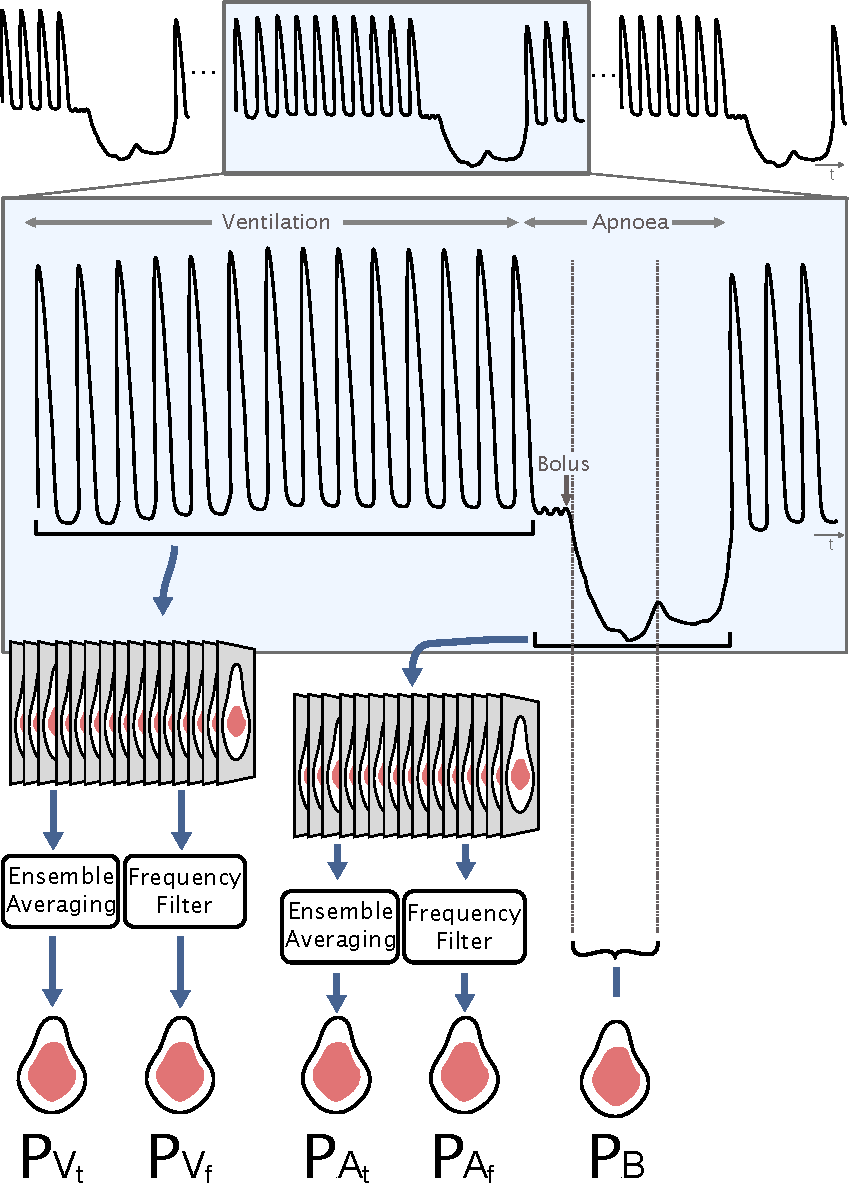
\includegraphics[width=0.8\textwidth]{chapter_2/imgs/fig-methodsOverview.pdf}
\end{flushright}
\caption{\label{fig:methods}%
This figure is a schematic overview of analysis methods for EIT perfusion. 
The upper
curve illustrates the global EIT signal during a period of ventilation
followed by apnoea and renewed ventilation. During apnoea a bolus
of conductivity contrasting saline is introduced. From these data
5 fEIT images are calculated:
$\PVa$: pulsatility (perfusion) image during ventilation, calculated
by ensemble averaging EIT data during ventilation;
$\PVi$: pulsatility (perfusion) image during ventilation, calculated
by frequency filtering EIT data during ventilation;
$\PAa$: pulsatility (perfusion) image during apnoea, calculated
by ensemble averaging EIT data during apnoea;
$\PAi$: pulsatility (perfusion) image during apnoea, calculated
by frequency filtering EIT data during apnoea;
$\PBi$: perfusion image from bolus, calculated between a 
reference measure during apnoea and one during the bolus}
\end{figure}

\subsection{Data Acquisition and Image Reconstruction}

EIT data was acquired with the Pioneer Set (Swisstom, Landquart, Switzerland)
using a custom electrode belt (at an acquisition rate of 20\,frames/s).
The belt uses 32 brass electrodes equally spaced around the thorax, 
using an ultrasound gel to ensure good contact and minimise the contact impedance. 
The selected data in this study comes from lateral positioning changes recorded after
after 1.5 hours of ventilation and prone to supine positioning changes after 
2 hours.

EIT images were 
reconstructed using GREIT \parencite{Adler2009}, %(Adler \etal 2009), 
which
calculates a reconstruction matrix $\RB$ from which
the reconstructed image is calculated as $\xH = \RB \yB$,
where $\yB$ are the time-difference
measurements,
$\yB(t) = \vB(t) - \vB(t_r)$,
where $\vB(t)$ represents 
the data frame acquired at time, $t$,
and $\vB(t_r)$ measurements acquired at a 
``reference'' time, $t_r$ 
in the case of this experiment the reference was
a mean of 10 images preceding the bolus injection.

The linear reconstruction matrix $\RB
 = \DB \SG_t \JB^T 
    \left(
       \JB \SG_t \JB + \SG_n
    \right)^{-1}
$ is calculated from a
finite element model of the body and electrode geometry
$F(\cdot)$ and covariance estimates of the image, $\SG_t$, 
noise, $\SG_n$ \parencite{Grychtol2016}, %(Grychtol \etal 2016), 
and
a spatial filtering matrix, $\DB$.

EIT data from this experiment was prone to errors consisting of brief 
periods of zeroed measurements stemming 
from the synchronisation equipment. 
Measurements that were zeroed by the device were removed and replaced with linearly  
extrapolated data to allow for frequency-based analysis over all selected segments
of data.
A moving median filter with a width of 3 was used to further remove the
noise caused by single measurement errors in the signal.

%Data that was selected required preprocessing 
%to identify and compensate for
%measurement errors. Ventilation regions 
%were selected as time series segments of data, 
%20 seconds in length, immediately preceding the onset of apnoea.
%
%The entire apnoea section was used unless a
%recording error occurred during this time where the EIT system 
%recorded no data. All 
%recording errors were identified and removed so they did not 
%affect the reconstruction reference level or the resulting images.
%To eliminate these measures, elements of the noise covariance matrix $[\SG_n]_{i,i}$, 
%corresponding to error measurements were set to 
%a large value to
%indicate a high level of noise, and to reduce the impact on the resulting
%image.

\subsection{Functional EIT Images}

In each animal 4 episodes were recorded --- one in each posture --- to generate 5
different functional EIT images. 

The images
Bolus-based measures of lung perfusion ($\PBi$) were
calculated using time-difference
reconstructions. Heart-frequency filtering during ventilation ($\PVi$) and
apnoea ($\PAi$) used
frequency analysis of EIT image sequences, as 
illustrated in \fref{fig:freqAnalysis}, and ensemble averaging-based methods during ventilation
$\PVa$ and apnoea $\PAa$ are 
calculated using ensemble averaging of identified pulsitile components~\fref{fig:timeAnalysis}.

The following methods were conducted on segments of data collected both during apnoea and ventilation. 
Apnoea regions were selected as the total time that ventilation was arrested, including the bolus section
and had a duration of 30s. The ventilation data was selected as 30s of data immediately preceding the 
induction of apnoea.
Regions of interest including lung, and heart areas in the images were defined by the lamb model
provided in EIDORS~\parencite{Adler2017b}.

\subsubsection{Bolus injection image $(\PBi)$}

The beginning of the saline bolus injection was determined as the point
immediately preceding the drop in impedance from the conductive agent, and is
shown in~\fref{fig:methodsBolus} at the point marked ``injection''.
The mean of 10 images including and immediately preceding the bolus injection were used 
as the reference to which all bolus images were reconstructed from. 
To image perfusion, the point with maximum decline in impedance over 
the sum of the pixels in the lung region relative to the reference was selected based on the methods 
presented by \citeauthorandyear{Frerichs2002}.
In~\fref{fig:methodsBolus} this was found at the point marked ``perfusion''. 
This method was used as the standard perfusion 
measuring technique
against which the other methods were compared.

\begin{figure}
\begin{flushright}
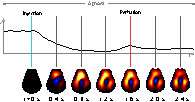
\includegraphics[width=0.8\textwidth]{chapter_2/imgs/fig-methodsBolus.pdf}
\end{flushright}
\caption{\label{fig:methodsBolus}%
The method used to select the perfusion point from the bolus injection is shown 
in the figure above. The point with the widest spread of high conductivity was 
selected as the point of perfusion, shown here at 1.6 seconds after the contrast 
agent injection. The image series shows the conductivity contrast as the bolus 
injection travels through the thorax.
}
\end{figure}


\subsubsection{Frequency-Filtering} \label{freqVent}

Heart-frequency EIT images during the selected events were calculated 
by taking the FFT of the time-series image data after first applying a Blackman window: 
$w(n)=a_{0}-a_{1}\cos \left({\frac {2\pi n}{N-1}}\right)+a_{2}\cos \left({\frac {4\pi n}{N-1}}\right)$ 
with $a_{0} = 0.42$, $a_{1} = 0.5$ and $a_{2} = 0.08$, where N is the number of time-series 
EIT images in the selected event.

An FFT was calculated from a series of images restricted to pixels in the heart 
region. From the FFT 
of all pixels the heart region, the heart frequency was selected as the largest 
peak between 3 and 4.5 Hz, representing a heart rate between 180 
and 240 bpm (typical for a newborn lamb).

The identified heart rate was used to select changes at the heart-frequency 
in the frequency domain images of the entire thorax. 
Images at 3 frequencies on either side of the heart rate were also reconstructed 
to account for changed in heart rate over the course of the data collection.
A Blackman window with a length of 7 was applied 
surrounding the heart frequency to generate a weighted mean of the images, resulting in 
a single perfusion image from the heart-frequency data. 
 
The output of the frequency filtering method is an 
image with complex values assigned to each pixel.  

Depending on the timing of the pulsatility-based changes within the selected signal
the real component of frequency analysed image 
did not correspond to the maximum conductivity 
change in the lungs in every event.
In order to correct this, each image was displayed along the axis that gave the maximum real component contained
within the lung region to ensure
the maximum change in impedance related to pulsatile activity in the lungs was calculated.

\begin{figure}
\begin{flushright}
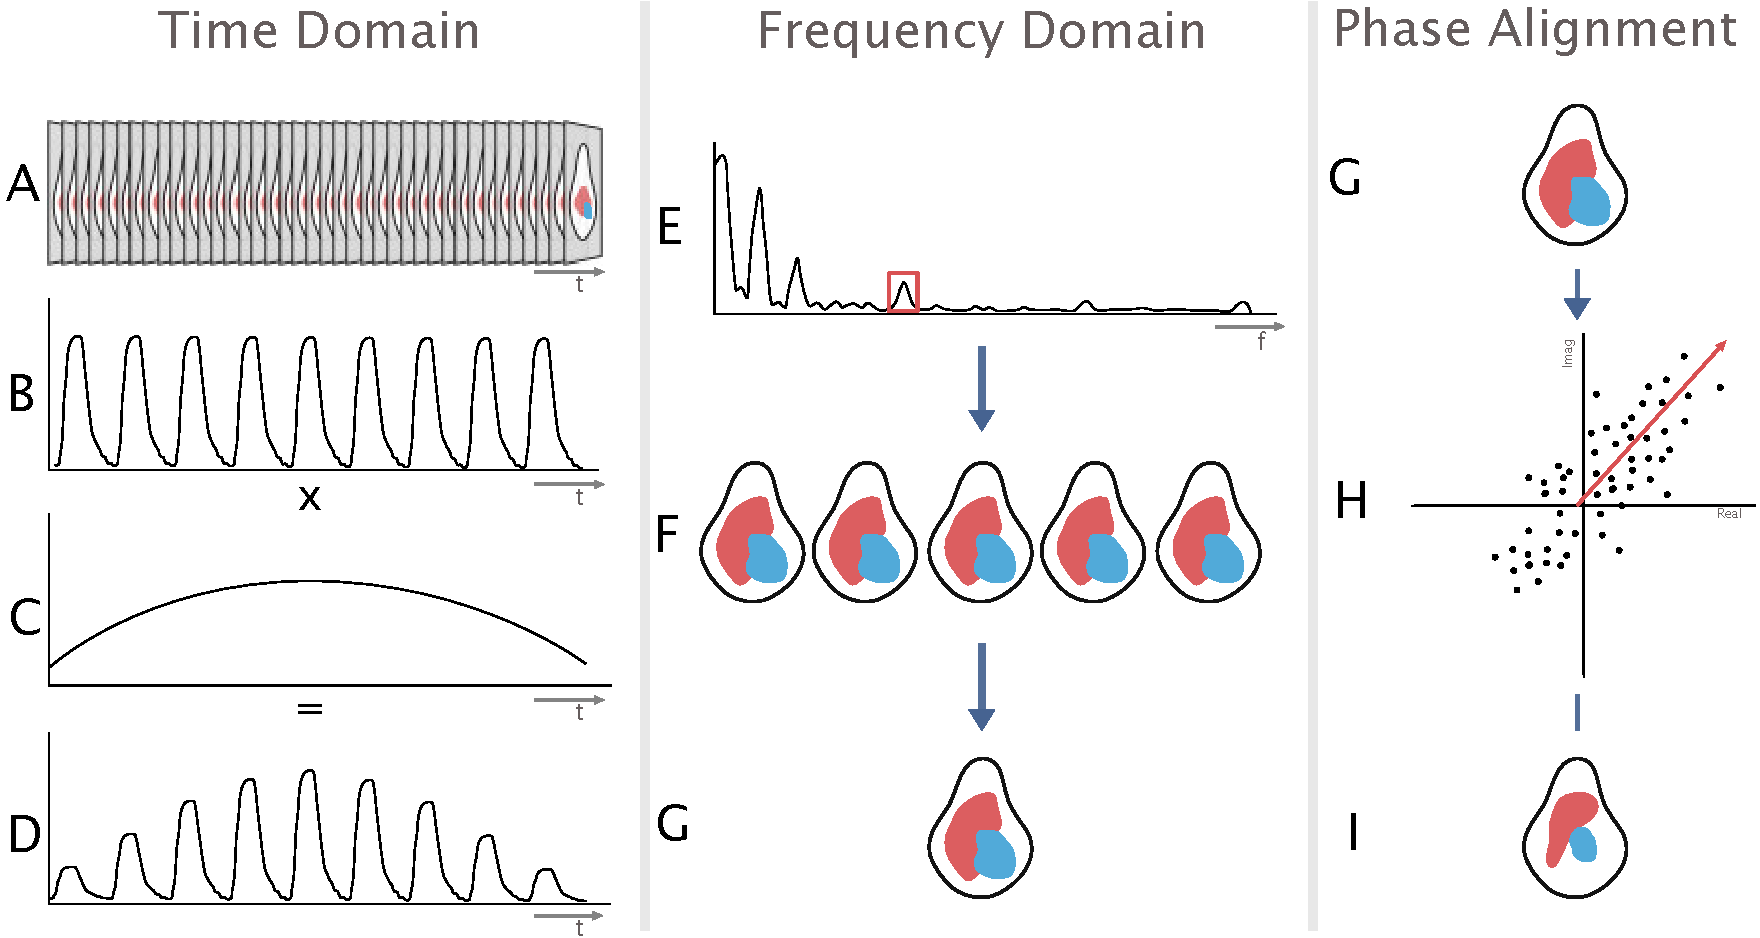
\includegraphics[width=0.8\textwidth]{chapter_2/imgs/fig-methodsFrequency.pdf}
\end{flushright}
\caption{\label{fig:freqAnalysis}
Frequency analysis methodology used for obtaining a perfusion image 
from the time series data. Steps are: 
A) to reconstruct the images from time series measurements; 
B) - D) window the time series data before performing a 
FFT on the data for each element; 
E) Select the dominant frequency between 3 and 4.5 Hz as the heart frequency;
F) reconstruct the image at the heart frequency and selected nearby frequencies; 
G) take the mean of the images at the heart frequency using a Blackman window 
to give greater weight to those closer to the center; 
H) I) select the image that will give the maximum real component contained
in the lung region.
}
\end{figure}

\subsubsection{Ensemble Averaging}

Time series data of the total impedance signal for each pixel in the heart region was filtered 
using a bandpass filter to eliminate noise and breathing changes, 
and allow the heartbeat to be seen clearly in the signal.
Peak detection was used on this heart-region data
to select the amplitude peaks in impedance change
signal at the heart frequency.

Using the identified time points, the global impedance change signal 
was ensemble averaged by overlaying all identified peaks 
to give an averaged heartbeat. 13 images were reconstructed over the 
course of the heart beat to select the image that resulted in the maximum 
positive increase impedance within the lung region. This process is outlined 
in~\fref{fig:timeAnalysis}.

\begin{figure}
\begin{flushright}
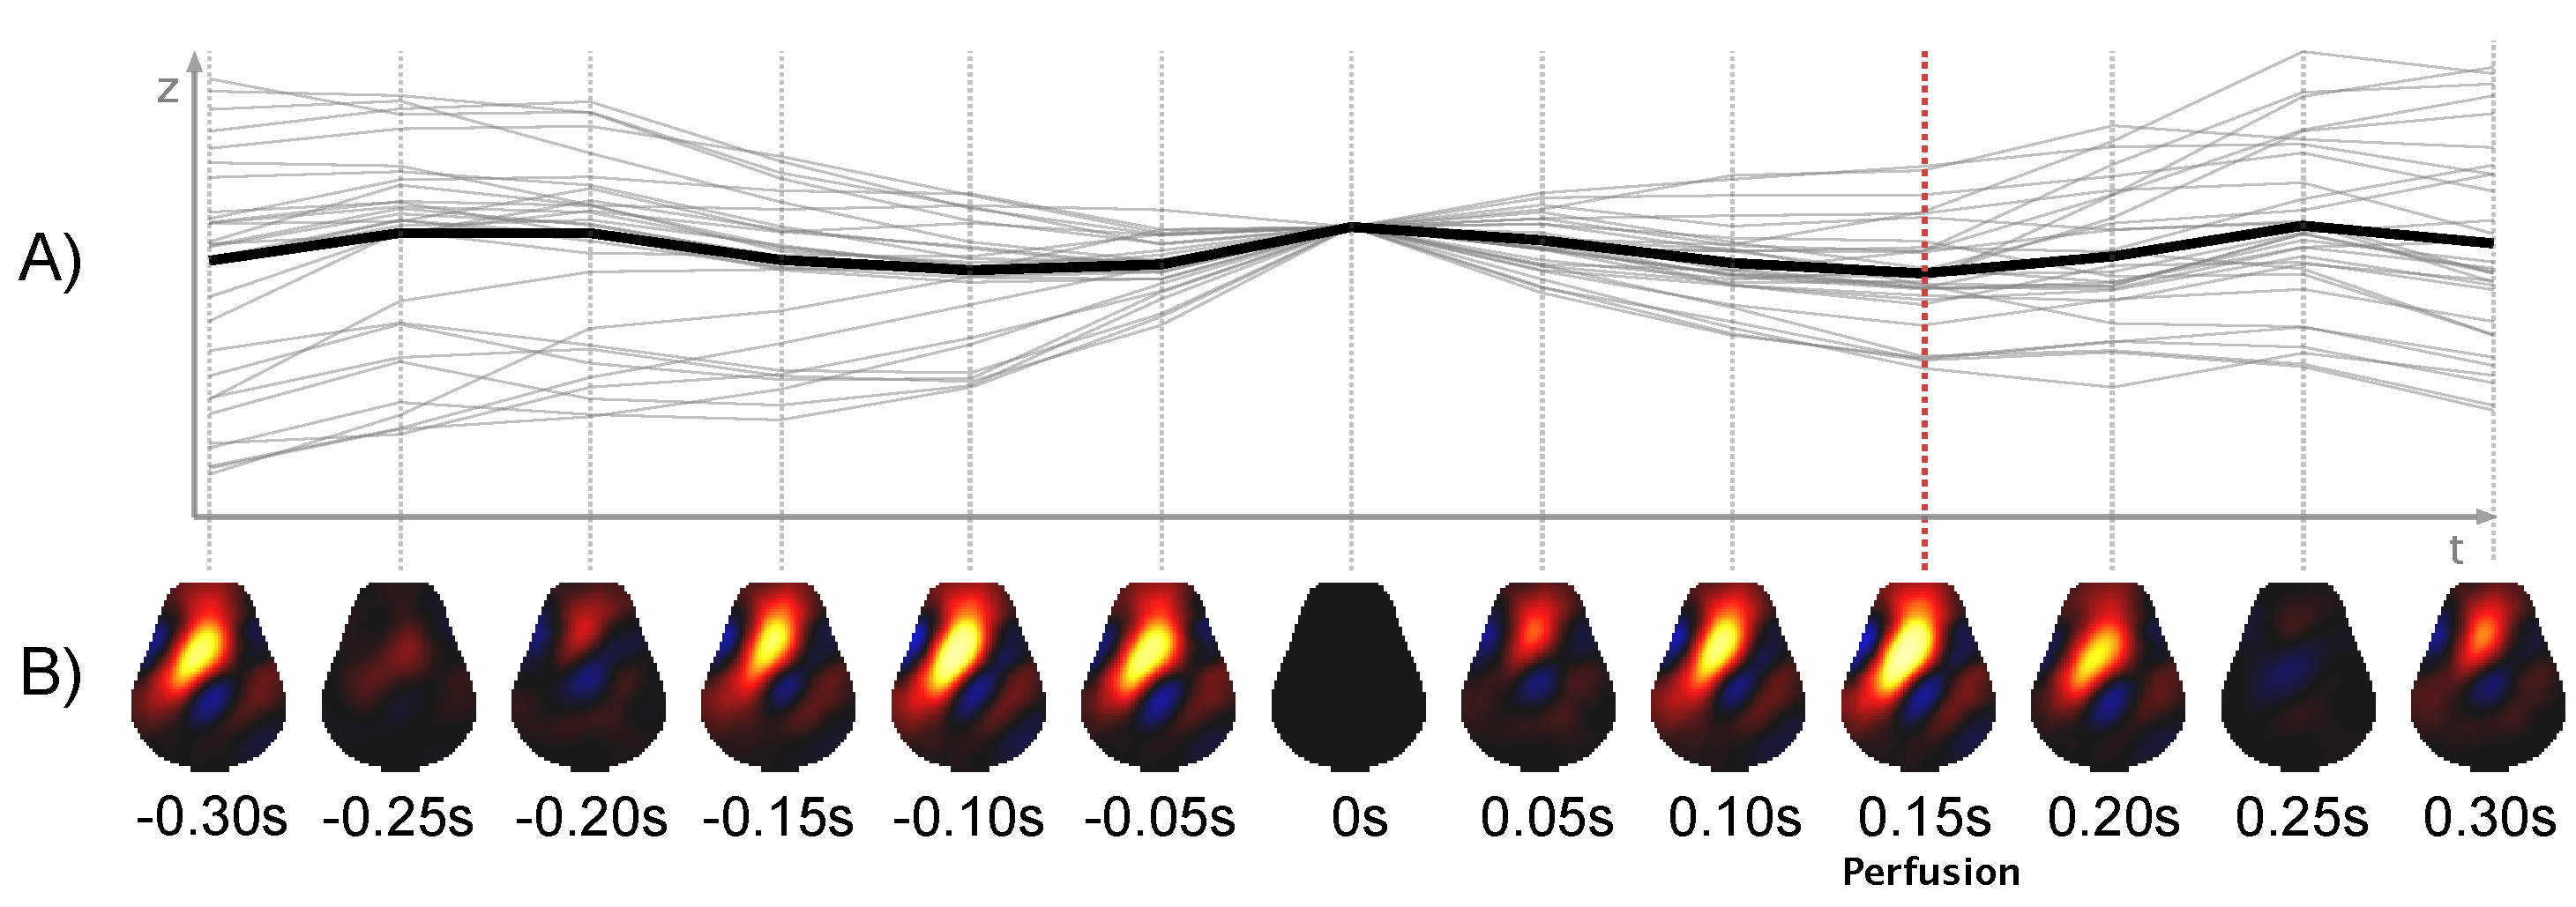
\includegraphics[width=0.8\textwidth]{chapter_2/imgs/fig-methodsTime.pdf}
\end{flushright}
\caption{\label{fig:timeAnalysis}%
Illustration of the stages of the ensemble averaging process:
A) an ensemble average of all heartbeats over the time frame is taken from the 
summed global signal; and 
B) shows reconstructed images corresponding to each time point 
in the global ensemble averaged signal above.
The selected perfusion image is the image with the maximum impedance increase in the 
lung region.
}

\end{figure}

\subsection{Image Comparison}

To compare the images the Jaccard 
distance between functional EIT images was calculated. 
Negative impedance changes were removed from the images
and the images were normalized.

The Jaccard distance was calculated between the reference image 
calculated using the maximum increase in lung-region conductivity during 
bolus injection (b), and the frequency-based method (f):
$J(x,y) = \sum_{i}\frac{min(b_i,f_i)}{max(b_i,f_i)}$
representing the distance between the two images.

\subsection{Statistical Analysis}

To determine the significance of the change in bolus between postures
and methods, the Cohen's d score was calculated to quantify the effect size of
the change in the centre of mass of the perfusion image~\parencite{Cohen1988}.  
This was calculated as the difference between two means over the pooled standard deviation. 
Where the difference between the two means is: $\mu_1-\mu_2$, and the pooled
standard deviation is: ${\sqrt{\frac{(n_1-1)s^2_1+(n_2-1)n_2s^2_1}{n_1+n_2-2}}}$. 

\section{Results}                         %% RESULTS %%

The Jaccard scores for each method were compared between 
ensemble averaging and frequency filtering methods to determine the regions where performance 
was best for each method. Figure \ref{fig:resultsJaccard} shows a 
comparison between Jaccard distance for each animal, connecting lines 
indicate different methods performed on the same data segment, while each marker shape
denotes a separate posture.

\begin{figure}
\begin{flushright}
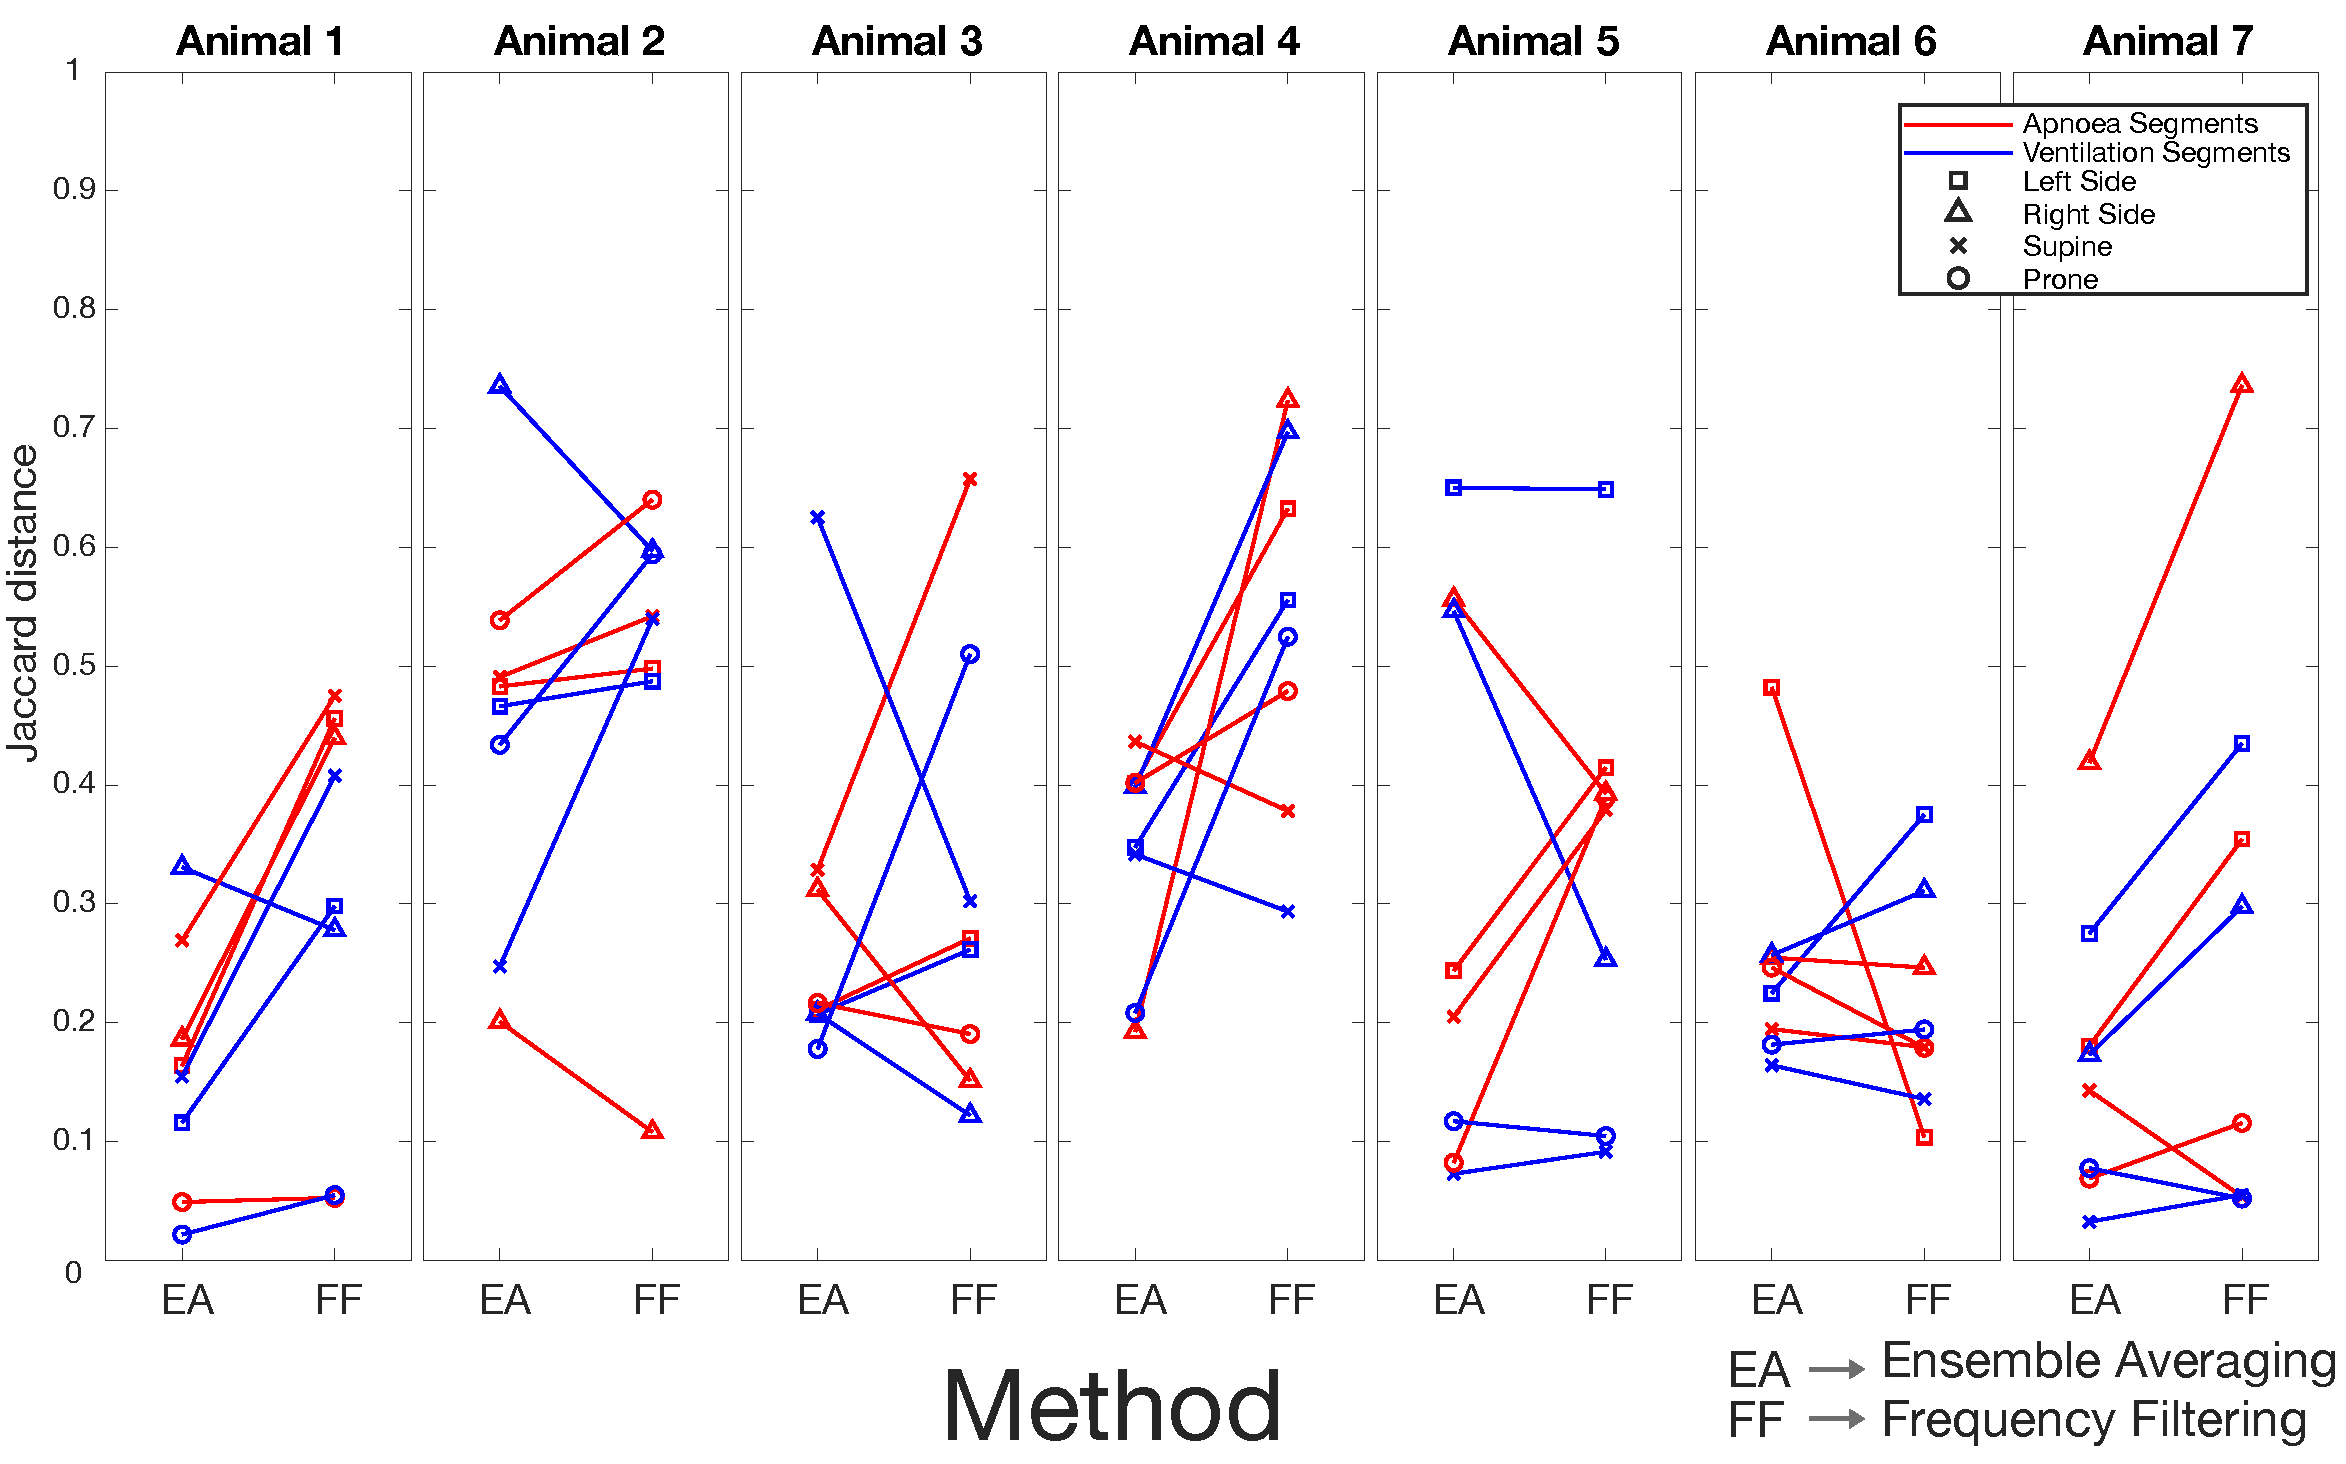
\includegraphics[width=0.8\textwidth]{chapter_2/imgs/fig-resultsJaccard.pdf}
\end{flushright}
\caption{\label{fig:resultsJaccard}%
Jaccard scores for each method and animal in the comparison. Frequency 
filtering and ensemble averaging methods performed on the same data segment are 
connected by solid lines. Red lines and markers indicate apnoea data sections, 
while blue indicates ventilation data sections. Each posture is denoted by a different
shaped marker in the figure.
}
\end{figure}

On average frequency filtering outperforms ensemble averaging based methods
of perfusion calculation (p=0.04), and there is no significant difference in
performance of the heart-frequency based 
filtering techniques during periods of apnoea relative to periods of ventilation.

Of the 56 data regions that were analysed,
the ensemble averaging performed better in 12 cases and the frequency 
filtering achieved the best performance in 28 cases, there, were 16 additional cases 
where the difference in performance was negligible at less than 5\%. On 
average, across all images, frequency filtering based methods scored
7\% higher than ensemble averaging.

The center of mass of the perfusion 
measure images using the bolus injection method had a Cohen's d score of less than 0.1 
between posture changes
indicating that there is an insignificant or trivial difference in the means relative
to the standard deviation \parencite{Cohen1988}. 
To demonstrate the visually observable changes due to posture change and the 
high similarities that can be observed between filtering- and bolus-based 
perfusion estimates, frequency filtered images from 
animal 4 are compared to bolus based methods in \fref{fig:discussionSample}.

\begin{figure}
\begin{flushright}
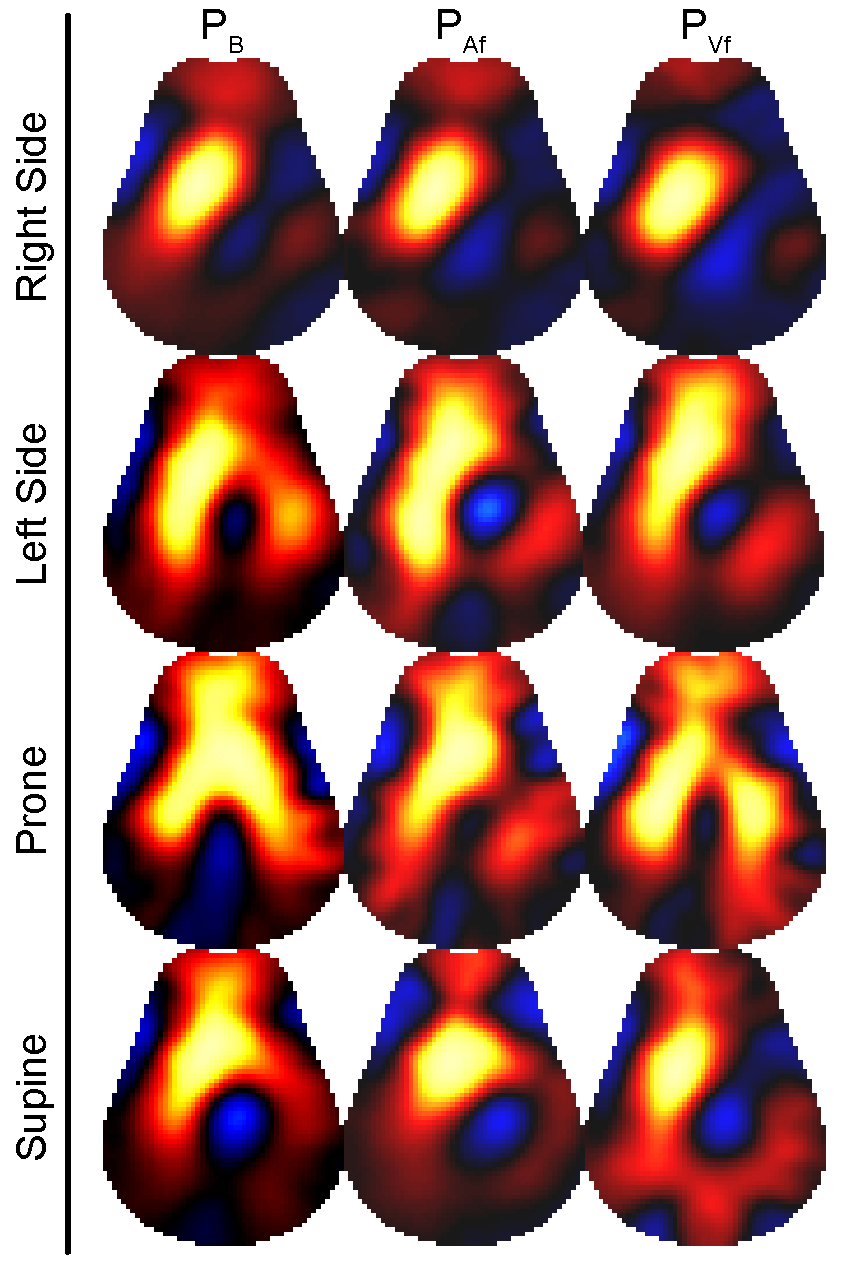
\includegraphics[width=0.7\textwidth]{chapter_2/imgs/fig-discussionSample.pdf}
\end{flushright}
\caption{\label{fig:discussionSample}%
		This figure shows the tracking of perfusion for frequency filtering measures
		of perfusion during apnoea and ventilation sections compared to bolus injection
		for animal 4.
$\PBi$ is the bolus injection image, 
$\PAi$ uses the frequency filtering method during apnoea and
$\PVi$ is the frequency filtering method during ventilation.
}
\end{figure}

\section{Discussion}                             %% DISCUSSION %%

Two primary approaches of EIT perfusion calculation
have been compared in this paper: injection
of a bolus of contrast-agent resulting 
in EIT image changes which produce perfusion measures, and
digital filtering of EIT image sequences to extract
the heart-frequency components.
Additionally, various algorithms have been evaluated
for digital filtering-base approaches during mechanical 
ventilation and short apnoea sequences, 
using both frequency- and ensemble averaging-based techniques.
There have been few comparisons of
these techniques, and 
we set out to better understand the relationship between
perfusion and heart-frequency measures, and between the various filtering
approaches used to determine heart-frequency cardiac changes.
We selected an experimental protocol using posture-change 
to alter the regional distribution of lung ventilation
and perfusion in newborn lambs.

Our first question was
``to what extent do heart-frequency filtering-based measures correspond to perfusion?''

The primary results (\fref{fig:resultsJaccard}) use a Jaccard index of the similarity
between functional images. Overall it was found that in healthy animals 
the Jaccard index indicated good agreement with our gold standard. While highly
dependant on the data, it was found that there was a high degree of similarity 
between methods with respect to
the overall shape of the perfusion. 
In both animals 2 and 4, where the signal required little preprocessing before analysis 
there is a higher Jaccard score across all cases.

The synchronisation box was attached to the EIT system but was not used for this experiment,
an error in the connection caused brief periods of the signal (less than 1\,s) in some animals to be zeroed.
Through careful processing of this signal only brief sections of data were lost and we do not feel this
impacts the results.

% Limitations
During the experiment the order of posture change was not randomised. 
While changes in ventilation due to posture change
are not understood to have long term physiological effects, if there is a longer term
effect of change in posture the lack of randomisation will impact the results. 
\citeauthorandyear{Nguyen2015} were able to image perfusion changes due to induced 
pulmonary embolisms and using the peak impedance change on dilution curves,
however our data presented insufficient variance in perfusion induced by posture change to 
complete a center of mass analysis. A higher statistical power 
could potentially be achieved through initiating posture changes
with more dramatic results in perfusion, such as upright to supine \parencite{Nakazato2010}.

Throughout the experiment, 
the perfusion image was selected as the image containing 
the largest increase in conductivity in the sum of pixels 
in the lung region, which occurred 
at different relative times across animals and events. Many factors could affect this
including belt positioning changes, and it could be a contributing factor 
to the inconsistent trends in amplitude changes in the global image across methods.
\citeauthorandyear{Borges2012}
compared EIT perfusion images using first-pass kinetics and 
heart-frequency filtering based methods to perfusion measures using SPECT,
finding that heart-frequency filtering
techniques made systemic errors when used to estimate the perfusion. They also 
determined that there was no discernible relationship between the magnitude of the
SPECT images and the heart-frequency images.
This was consistent with the findings of this study that image amplitude of the bolus injection and 
heart-frequency filtering-based methods was not consistent in all animals.
This methodology presented by \citeauthorandyear{Borges2012}
was not part of the comparison in this study as the edentification of the 
perfusion signal due to the heart could not be consistently
identified and removed across all animals.
In two dimensions, heart-frequency and ventilation signals 
have been used to identify the location 
of the heart and lungs within the EIT electrode plane with known electrode 
locations and anatomy~\parencite{Ferrario2012}, but in situations where the electrode 
location and anatomy is not precisely known EIT tends to perform poorly as a structural 
imaging modality~\parencite{Adler2017a}.
These challenges suggest that configurations with multiple planes of electrodes 
may be better able to isolate and remove off-plane 
pulsatility signals related to the heart.

It was observed that the general shape of 
the perfusion was consistent across all methods despite amplitude variations. 
One reason for the difference in amplitude change across animals may be due 
to slight variations in the belt placement and electrode positioning on the animals.
If the belt is closer to the heart, there will be a larger heart-frequency component 
to the signal and there may be a variance in the impedance change due to bolus injection.

Next, we asked ``what are the advantages and disadvantages of different approaches
to heart-frequency filtering of EIT data, and which techniques are recommended
under which circumstances?''

Our overall recommendation is that, whenever possible, 
frequency filtering techniques should be used. This is largely
because frequency filtering methods tend to be more stable in the 
presence of noise on the signal. 
Ensemble techniques are advantageous
in some circumstances, because they better use the heart-frequency
variability to avoid interference from harmonics of the
ventilation at the heart rate. For frequency-filtering
techniques, it is necessary to widen the heart-frequency
filters to account for such variability.
On the other hand, it is sometimes not possible to accurately
synchronize heartbeats, due to noise corruption in the
signals or the very low amplitude of the heart-frequency signals
relative to the ventilation signal.
In cases where the signal of the heartbeat 
was not clearly identifiable through visual inspection of the signal, neither 
ensemble averaging nor frequency filtering was able to achieve good 
estimates of perfusion relative to the bolus injection event. 

In summary, 
our goal was to understand the relationship between bolus- and filtering-based
EIT measurements of lung perfusion, as well as the relationship between different
filtering-based measures of perfusion.
Our results indicate there is a common trend between the shape and perfusion  
estimates of both heart-frequency and bolus injection images 
despite the difference in physiological events behind each measure.
Amongst filtering techniques, frequency
filtering outperforms ensemble averaging across regions of data where there is noise present and the 
heart signal cannot be readily identified, and both methods were able to approximate the bolus injection 
measures equally well when applied to apnoea and ventilation regions of data.

%\include{chapter3/chapter3_body}
%\include{chapter4/chapter4_body}
%\include{chapter5_body}
%\include{chapter6_body}

% BIBTEX
\markboth{Bibliography}{Bibliography}
\addcontentsline{toc}{chapter}{Bibliography}
%\bibliography{/home/cgomez/Documents/thesis/references/thesis}
\begin{singlespace}
  \setlength\bibitemsep{2pt}
  \printbibliography
\end{singlespace}

\appendix 
\include{appendix/appendix_body}


\end{document}
